\documentclass[12pt]{article}

\usepackage[margin=1in]{geometry}
\usepackage{setspace}
\usepackage{graphicx}
\usepackage{amsmath}
\usepackage{amssymb}
\usepackage{array}
\usepackage{booktabs}
\usepackage{tabularx}
\usepackage{threeparttable}
\usepackage{listings}
\usepackage{xcolor}
\usepackage{float}
\usepackage[
  backend=biber,
  style=apa,
  natbib=true,
  sortcites=true,
  sorting=nyt,
  doi=true,
  url=true,
  isbn=false
]{biblatex}
\usepackage{tikz}
\usepackage{fancyhdr}
\usepackage{microtype}
\usepackage[hidelinks]{hyperref}
\usetikzlibrary{arrows.meta,positioning,fit}

\IfFileExists{reference.bib}{%
  \addbibresource{reference.bib}%
}{%
  \addbibresource{outputs/reference.bib}%
}

\doublespacing
\setlength{\parindent}{0.5in}
\setlength{\parskip}{0pt}
\setlength{\headheight}{15pt}
\setlength{\emergencystretch}{2em}

\pagestyle{fancy}
\fancyhf{}
\fancyhead[R]{\thepage}
\renewcommand{\headrulewidth}{0pt}

\newcommand{\pkg}[1]{\texttt{#1}}
\newcommand{\code}[1]{\texttt{#1}}
\newcommand{\fcode}[1]{\nolinkurl{#1}}
\newcommand{\todo}[1]{\textbf{[TO DO: #1]}}
\newcommand{\maybegraphic}[2][\linewidth]{%
  \IfFileExists{#2}{%
    \includegraphics[width=#1]{#2}%
  }{%
    \IfFileExists{outputs/#2}{%
      \includegraphics[width=#1]{outputs/#2}%
    }{%
      \fbox{\parbox[c][1.7in][c]{0.90\linewidth}{%
        \centering Figure file to be supplied at submission:\\
        \texttt{\detokenize{#2}}}}%
    }%
  }%
}

\lstset{
  language=R,
  backgroundcolor=\color{white},
  basicstyle=\footnotesize\ttfamily,
  breaklines=true,
  captionpos=b,
  keepspaces=true,
  numbers=left,
  numberstyle=\tiny\color{gray},
  stringstyle=\color{purple},
  commentstyle=\color{gray},
  keywordstyle=\color{blue},
  showstringspaces=false,
  frame=single,
  framerule=0.2pt,
  xleftmargin=1.5em,
  framexleftmargin=1em
}

\title{\pkg{BERTopic} for R: An Interface to the Python Implementation for Behavioral Research Workflows}

\author{
Biying Zhou\textsuperscript{1},
Yuhao Yuan\textsuperscript{1},
Nanxin Deng\textsuperscript{2},
and Feng Ji\textsuperscript{1}\\[0.5em]
\textsuperscript{1}\todo{Affiliation}\\
\textsuperscript{2}\todo{Affiliation}\\[0.5em]
\parbox{0.82\textwidth}{\centering
\todo{Corresponding author name, postal address, telephone number, and email}}
}

\date{}
\begin{document}

\maketitle
\thispagestyle{fancy}

\begin{abstract}
BERTopic provides an embedding-based approach to topic modeling, but its implementation and compatible machine-learning components are maintained primarily in Python. R users can connect to that ecosystem through general-purpose interoperability code or dedicated packages, although the resulting workflows still require explicit management of Python environments, object conversion, and model state. We describe \pkg{BERTopic}, an open-source R interface that retains the fitted Python model while exposing common operations through an S3 object, R functions, tibbles, and matrices. An SMS example illustrates environment selection, fitting, inspection, prediction, export, visualization, and persistence. We also tested whether the wrapper preserved selected outputs from equivalent direct Python code. Five paired fresh-process runs used the same 2,247 documents and frozen five-dimensional reduced embeddings, with identically configured components, software versions, and process settings. The two paths returned identical assignments, metadata, and ordered term keys; weights and membership-strength matrices agreed within an absolute tolerance of 1e-12. In this controlled Windows task, paired R-minus-Python differences had medians of 4.183 seconds for fitting, 11.400 seconds for cold-process time, and 200.0 MiB for peak memory. Because embedding generation and UMAP fitting were excluded, these measurements describe the additional costs of the tested R workflow rather than complete BERTopic performance. The contribution is an R-oriented access layer and a validation of its tested fitting and extraction path, not a new topic model or an independent implementation of BERTopic.
\end{abstract}

\noindent\textbf{Keywords:} topic modeling; BERTopic; R package; Python interoperability; behavioral text analysis; research software

\section{Introduction}

Behavioral researchers use open-ended survey responses, interviews, online discussions, clinical notes, and administrative records to study information that may be difficult to capture with closed-response measures. Exhaustive manual coding becomes costly as these collections grow. Topic models provide one way to summarize recurring patterns and construct document-level representations for subsequent qualitative inspection or quantitative analysis \citep{blei2003latent,grimmer2013text,roberts2014structural}.

Classical methods such as latent semantic analysis, probabilistic latent semantic analysis, non-negative matrix factorization, and latent Dirichlet allocation represent documents primarily through word occurrence patterns \citep{deerwester1990latent,hofmann1999plsa,lee1999nmf,blei2003latent}. Transformer models instead provide contextual representations in which documents with different surface forms can occupy nearby regions of an embedding space \citep{vaswani2017attention,devlin2019bert,reimers2019sentence}. Embedding-based topic-modeling systems use this geometry to organize documents before deriving human-readable topic descriptions, which can be useful for short or lexically heterogeneous text \citep{angelov2020top2vec,bianchi2021pretraining}.

BERTopic is a modular framework in this family \citep{grootendorst2022bertopic}. Its default workflow combines contextual embeddings, UMAP dimensionality reduction \citep{mcinnes2018umap}, HDBSCAN clustering \citep{campello2013density,mcinnes2017hdbscan}, and class-based TF--IDF (c-TF--IDF) topic representations. Researchers can replace these components, but the official implementation and the compatible embedding and clustering ecosystem are maintained primarily in Python.

This dependence on Python can complicate projects in which data management, statistical analysis, visualization, and reporting are conducted in R \citep{rcore2026}. R supports text-analysis workflows through \pkg{tm}, \pkg{tidytext}, and \pkg{quanteda} \citep{feinerer2008tm,silge2016tidytext,benoit2018quanteda}. Researchers can exchange files between R and Python or write \pkg{reticulate} code, although either route requires decisions about Python selection, argument passing, object conversion, and error diagnosis \citep{ushey2026reticulate}. Dedicated R interfaces have also emerged. In particular, \pkg{bertopicr} provides helpers for Python-environment setup, model training, persistence, inspection, and visualization \citep{petric2026bertopicr}. The relevant question is therefore not whether an R interface exists, but how a particular interface organizes the workflow, which backend versions it supports, and which operations have been tested.

The R interface does not change BERTopic's statistical model. Its purpose is to call the official implementation from R and return selected results in forms that can be used in later R analyses. Evaluating whether the wrapper passes inputs and outputs correctly is separate from evaluating whether BERTopic produces substantively valid topics for a particular corpus.

We present \pkg{BERTopic}, an alternative R interface to the Python implementation. Its design emphasizes a retained Python model inside an S3 object, familiar methods such as \code{predict()}, \code{coef()}, \code{as.data.frame()}, and \code{fortify()}, explicit dense or sparse export, and functions for selecting and diagnosing the Python environment. A worked example demonstrates the intended workflow. We then compare the R call with equivalent direct Python code under a controlled configuration and report output agreement together with descriptive runtime and memory measurements. This comparison examines the wrapper's handling of selected inputs and outputs; it is not a comparison of two topic-modeling algorithms, a feature-completeness study of R packages, or a validation of the substantive topics recovered from the SMS corpus.

\section{Computational Background and Scope}

\subsection{Scope of the R package}

The Python library performs document embedding, dimensionality reduction, clustering, vectorization, topic weighting, and optional refinement of topic labels. The R package validates inputs, calls Python through \pkg{reticulate}, stores the fitted Python object, and converts selected results to R objects. It also provides functions for installing and selecting a Python environment, checking dependencies, and saving fitted models. The statistical properties of the fitted model remain those of the Python library and the component models chosen by the user.

The following summary describes the BERTopic pipeline only to show how the R functions correspond to the Python implementation. The worked example demonstrates use of the package. The later comparison checks selected results against a direct Python call and measures runtime and memory use. Neither exercise establishes that the topics from an unsupervised model are substantively valid.

\subsection{The six-stage upstream pipeline}

The R package delegates computation to the upstream Python library. The default BERTopic workflow can be summarized in six stages:

\begin{enumerate}
    \item An \code{embedding\_model} converts documents into dense contextual vectors.
    \item A \code{umap\_model} or another compatible reducer projects the vectors into a lower-dimensional space.
    \item An \code{hdbscan\_model} or another compatible clusterer assigns documents to candidate topics and may identify outliers.
    \item A \code{vectorizer\_model} constructs topic-level term counts from the documents assigned to each cluster.
    \item A \code{ctfidf\_model} weights terms by their distinctiveness across topic-level document classes.
    \item An optional \code{representation\_model} refines, reranks, or relabels the topic representation.
\end{enumerate}

The resulting object combines document assignments, topic-level term representations, fitted component objects, and optional membership-strength information. The outlier topic is conventionally labeled \code{-1}. BERTopic is not a fully generative word-count model, and its probability output should not be interpreted as an LDA-style posterior topic mixture without additional justification.

\begin{figure}[htbp]
\centering
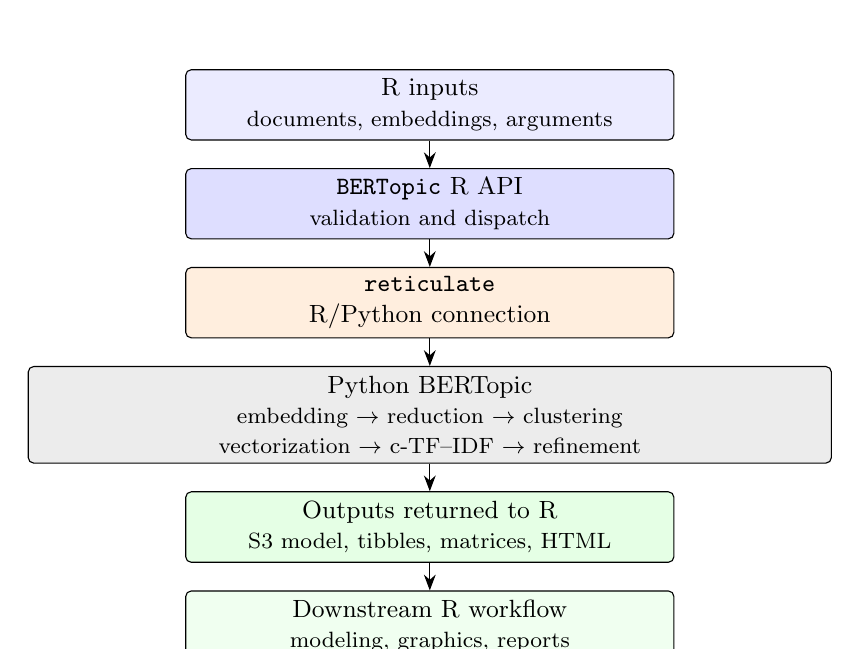
\begin{tikzpicture}[
    box/.style={
        draw,
        rounded corners=2pt,
        minimum height=0.82cm,
        align=center,
        font=\small
    },
    arrow/.style={-{Stealth[length=2mm]}, line width=0.45pt},
    node distance=0.35cm and 0.55cm
]
\node[box, fill=blue!8, minimum width=6.2cm] (rinput)
  {R inputs\\\footnotesize documents, embeddings, arguments};
\node[box, fill=blue!13, minimum width=6.2cm, below=of rinput] (rapi)
  {\pkg{BERTopic} R API\\\footnotesize validation and dispatch};
\node[box, fill=orange!13, minimum width=6.2cm, below=of rapi] (reticulate)
  {\pkg{reticulate}\\R/Python connection};
\node[box, fill=gray!15, minimum width=10.2cm, below=of reticulate] (python)
  {Python BERTopic\\\footnotesize embedding $\rightarrow$ reduction $\rightarrow$ clustering\\
  \footnotesize vectorization $\rightarrow$ c-TF--IDF $\rightarrow$ refinement};

\node[box, fill=green!10, minimum width=6.2cm, below=of python] (routput)
  {Outputs returned to R\\\footnotesize S3 model, tibbles, matrices, HTML};
\node[box, fill=green!6, minimum width=6.2cm, below=of routput] (workflow)
  {Downstream R workflow\\\footnotesize modeling, graphics, reports};

\draw[arrow] (rinput) -- (rapi);
\draw[arrow] (rapi) -- (reticulate);
\draw[arrow] (reticulate) -- (python);
\draw[arrow] (python) -- (routput);
\draw[arrow] (routput) -- (workflow);
\end{tikzpicture}
\caption{Architecture of the R interface. Core modeling is performed by the official Python library; the R package manages inputs, calls, conversion, and outputs returned to R.}
\label{fig:architecture}
\end{figure}

\subsection{Methodological scope}

The package does not reproduce UMAP, HDBSCAN, or c-TF--IDF in R. Their mathematical derivations are outside the scope of this paper and are available in the cited method papers and BERTopic documentation. Accordingly, the paper focuses on how arguments and objects are passed between R and Python, how Python environments are selected and checked, and whether selected outputs match those from a direct Python call.

\section{Software Design and Implementation}

\subsection{Relationship to other R interfaces}

The R packages \pkg{BERTopic} and \pkg{bertopicr} both connect R to the Python BERTopic ecosystem through \pkg{reticulate} \citep{petric2026bertopicr}. Their functionality overlaps: both support environment setup, model fitting, inspection, persistence, and visualization. The present package is organized around a \code{bertopic\_r} S3 object that retains the upstream model and adds familiar R methods, explicit conversion to common R data structures, and environment diagnostics. These design choices provide an alternative API rather than an independent statistical implementation.

This article evaluates selected input and output mappings against direct Python execution; it does not provide a head-to-head usability study or establish that one R package is generally preferable. Researchers should consider backend-version support, the operations required for their analysis, the available tests, and the preferred object model when choosing an interface. Table~\ref{tab:api_map} therefore documents the scope of \pkg{BERTopic}; it should not be read as evidence that every listed helper has received the same level of validation.

\subsection{R wrapper and model object}

The main entry point, \code{bertopic\_fit(text, embeddings = NULL, ...)}, calls BERTopic from an R session. The function validates that \code{text} is a character vector, checks that the Python library is available, imports the Python \code{bertopic} module, and forwards \code{...} to the Python \code{BERTopic()} constructor. If the user supplies a numeric R matrix of embeddings, the wrapper converts it to a Python-compatible array and passes it to \code{fit\_transform()}; otherwise, the configured Python embedding model creates the embeddings.

The return value has S3 class \code{bertopic\_r} and contains three main fields: \code{.py}, the fitted Python BERTopic object; \code{topics}, the document-level topic assignments returned during fitting; and \code{probs}, the membership-strength matrix when available. Storing \code{.py} gives users access to the complete fitted Python object. The wrapper converts common results to tibbles, R matrices, sparse matrices, or HTML files. Users can call the Python object directly for methods that do not yet have an R function.

Arguments supplied through \code{...} are passed to the Python constructor. Users may therefore create Python UMAP, HDBSCAN, vectorizer, c-TF--IDF, or representation objects with \pkg{reticulate} and pass them directly to \code{bertopic\_fit()}. This exposes BERTopic's configurable components within the backend versions explicitly supported by the R package. It does not guarantee forward compatibility with changed Python signatures. R also cannot validate every Python argument, so errors in advanced configurations may need to be diagnosed from the Python message and upstream documentation.

The retained Python object has reference semantics, whereas the wrapper's cached R fields are ordinary list elements. Updating topic representations changes the retained Python model in place. Topic reduction also changes assignments and membership strengths; callers must retain the returned wrapper, for example \code{model <- bertopic\_reduce\_topics(model, nr\_topics = 20L, docs = docs)}, to use the synchronized R fields afterward. This distinction matters for matrix exports, prediction, and persistence.

\subsection{Functions and return values}

Table~\ref{tab:api_map} summarizes the principal R functions, the Python operation they invoke, and the result returned to R. The functions cover model fitting, inspection, prediction, visualization, modification, and persistence.

\begin{table}[htbp]
\centering
\caption{Mapping Between the R Interface and the Python BERTopic Backend}
\label{tab:api_map}
\begin{threeparttable}
\small
\begin{tabularx}{\linewidth}{>{\raggedright\arraybackslash}p{3.8cm}
                             >{\raggedright\arraybackslash}p{3.4cm}
                             >{\raggedright\arraybackslash}X}
\toprule
R function & Python operation & R result or purpose \\
\midrule
\fcode{bertopic_fit()} & \fcode{BERTopic()}, \fcode{fit_transform()} & \fcode{bertopic_r} S3 object with retained Python model, assignments, and optional membership strengths \\
\fcode{bertopic_topics()} & \fcode{get_topic_info()} & Topic metadata as a tibble \\
\fcode{bertopic_topic_terms()} & \fcode{get_topic()} & Terms and c-TF--IDF weights as a tibble \\
\fcode{bertopic_find_topics()} & \fcode{find_topics()} & Query-nearest topic identifiers, scores, and labels \\
\fcode{bertopic_get_document_info()} & \fcode{get_document_info()} & Document-level metadata as a tibble \\
\fcode{bertopic_get_representative_docs()} & \fcode{get_representative_docs()} & Representative documents as a tibble; \fcode{top_n} limits the R result \\
\fcode{bertopic_transform()}\newline \fcode{predict()} & \fcode{transform()} & New-document assignments and optional membership strengths \\
\fcode{bertopic_as_document_topic_matrix()} & Stored fitting output & Dense or sparse R matrix for downstream analysis \\
\fcode{bertopic_update_topics()} & \fcode{update_topics()} & Updated topic representations \\
\fcode{bertopic_reduce_topics()} & \fcode{reduce_topics()} & Returned wrapper with synchronized assignments and strengths; requires reassignment \\
\fcode{bertopic_set_topic_labels()} & \fcode{set_topic_labels()} & Custom labels passed with integer topic keys \\
\fcode{bertopic_visualize_*()} & Python visualization methods & Interactive HTML output \\
\fcode{bertopic_save()}\newline \fcode{bertopic_load()} & \fcode{save()}, \fcode{load()} & Persistent fitted Python model wrapped for R reuse \\
\bottomrule
\end{tabularx}
\end{threeparttable}
\end{table}

The package also supplies S3 methods. \code{print()} and \code{summary()} provide compact model information; \code{predict()} presents transformation as a familiar prediction task; \code{coef()} returns top terms across topics; and \code{as.data.frame()} and \code{fortify()} support common R data workflows. These methods organize access to the fitted object but do not change its Python computations. Table~\ref{tab:api_map} lists the main functions. The controlled comparison in Section~\ref{sec:evaluation} covers only the fitting and extraction functions used in that test, not every helper in the table.

\subsection{Dependency management and diagnostics}

Because the package calls Python, backend installation is part of normal use. Version 0.1.2 provides Conda and virtualenv helpers and \code{install\_py\_deps()} as a dispatcher. Both routes consume the same exact requirements and run the same import validation. The supported tested configuration is Windows, Python 3.10.21, and BERTopic 0.16.0. Full resolved environments are retained with the outputs; other backend versions are outside this support claim.

The installation step is explicit rather than silently triggered by model fitting. Python machine-learning dependencies are large, may download model weights, and may require system-specific resolution. An explicit one-time operation makes this mutation visible. If the backend is missing, the fitting function stops with a diagnostic that names the active Python interpreter and the installation and binding calls required to continue.

Session binding is handled by \code{use\_bertopic()}, \code{use\_bertopic\_condaenv()}, and \code{use\_bertopic\_virtualenv()}. If \pkg{reticulate} has already initialized a different interpreter, these functions stop and instruct the user to restart the R session. This behavior avoids a common failure mode in which package installation succeeds in one environment but the R session imports from another.

Two functions support routine diagnosis. \code{bertopic\_available()} checks importability, while \code{bertopic\_session\_info()} reports the interpreter and exact versions for 11 key modules. Full Python distribution versions and R session information are also retained. The documented \code{bertopic\_self\_check()} fits, transforms, saves, loads, and compares cached fields, topic metadata, and post-load transformation outputs.

\section{Worked Example}

\subsection{Dataset and example plan}

This section demonstrates the main package functions using a 2,247-message subset of the UCI SMS Spam Collection included with the package \citep{sms_spam_collection_228}. Each row contains a binary label and one English SMS message. The packaged subset contains all 747 spam messages and 1,500 of the 4,827 ham messages in the source collection. \todo{Document the rule and random seed, if any, used to select the 1,500 ham messages, and archive a script that reconstructs the packaged data from the UCI source.} The labels are not used to fit the unsupervised topic model; they are retained to show the data structure and to support optional downstream checks. The direct comparison with Python is reported separately in Section~\ref{sec:evaluation}.

\begin{table}[htbp]
\centering
\caption{Structure and Descriptive Summary of the Packaged \code{sms\_spam} Data}
\label{tab:data_structure}
\begin{threeparttable}
\begin{tabularx}{\linewidth}{>{\raggedright\arraybackslash}p{2.1cm}
                             >{\raggedright\arraybackslash}p{2.1cm}
                             >{\raggedright\arraybackslash}X
                             >{\raggedright\arraybackslash}p{3.0cm}}
\toprule
Variable & R type & Role & Example or summary \\
\midrule
\code{label} & Character & Reference label; not supplied to BERTopic & 1,500 ham (66.8\%); 747 spam (33.2\%) \\
\code{text} & Character & One document per row; model input & ``Nah I don't think he goes to usf, he lives around here though'' \\
\addlinespace
\multicolumn{2}{l}{Document length} & Characters per message & Median = 84; IQR = 41--147; range = 2--790 \\
\multicolumn{2}{l}{Whitespace-delimited length} & Descriptive word count & Median = 16; IQR = 8--26; range = 1--162 \\
\bottomrule
\end{tabularx}
\begin{tablenotes}
\footnotesize
\item Note. Length statistics were computed before model fitting. The example text is reproduced from the packaged data.
\end{tablenotes}
\end{threeparttable}
\end{table}

The sequence covers environment diagnosis, fitting, inspection, semantic search, prediction, export, visualization, topic-representation updates, and persistence. It illustrates how the functions are intended to be combined; it is not a comparison of topic-modeling algorithms or evidence that topics recovered from this corpus represent behavioral constructs.

\subsection{Environment check and fitting}

The following code loads the data, creates the document vector, records the backend configuration, and explicitly fixes UMAP's random state. Setting only the global R or NumPy seed is not sufficient to make every stochastic component deterministic.

\begin{lstlisting}[caption={Checking the backend and fitting a BERTopic model from R.}]
library(BERTopic)
library(reticulate)

stopifnot(bertopic_available())
backend <- bertopic_session_info()

data("sms_spam", package = "BERTopic")
docs <- as.character(sms_spam$text)

set_bertopic_seed(42)
sentence_transformers <- reticulate::import("sentence_transformers", convert = FALSE)
embedding_model <- sentence_transformers$SentenceTransformer(
  "all-MiniLM-L6-v2", revision = "1110a243fdf4706b3f48f1d95db1a4f5529b4d41"
)
umap <- reticulate::import("umap", convert = FALSE)
umap_model <- umap$UMAP(
  n_neighbors = as.integer(15),
  n_components = as.integer(5),
  min_dist = 0,
  metric = "cosine",
  random_state = as.integer(42)
)

model <- bertopic_fit(
  text = docs,
  embedding_model = embedding_model,
  umap_model = umap_model,
  calculate_probabilities = TRUE
)
\end{lstlisting}

The number and composition of topics depend on the embedding model, reducer, clusterer, vectorizer, random state, and software versions. Users should therefore inspect the fitted object rather than expect the counts reported for the separate controlled evaluation below.

\subsection{Topic inspection and search}

\begin{lstlisting}[caption={Inspecting and querying the fitted topic solution.}]
topic_info <- bertopic_topics(model)
head(topic_info[c("Topic", "Count", "Name")], 8)

valid_topics <- topic_info$Topic[topic_info$Topic != -1]
bertopic_topic_terms(model, topic_id = valid_topics[1], top_n = 10)
bertopic_get_representative_docs(model, topic_id = valid_topics[1], top_n = 3)

bertopic_find_topics(
  model,
  query_text = "free subscription message",
  top_n = 5
)

document_info <- bertopic_get_document_info(model, docs)
head(document_info, 8)
\end{lstlisting}

Topic terms, counts, representative documents, and document-level information support inspection of the fitted solution. In the tested backend, \code{rank} identifies the order of returned representative documents; it is not a calibrated confidence score, and \code{top\_n} cannot request more documents than the backend retained. Researchers should inspect several documents per topic and document any coding or adjudication used to assign substantive labels. Automatic term-based names remain descriptions of cluster-specific patterns rather than validated behavioral constructs.

\subsection{Prediction and R-native export}

\begin{lstlisting}[caption={Transforming new documents and exporting training-corpus output.}]
new_docs <- c(
  "Love you so much, see you tonight.",
  "Free subscription! Reply STOP to unsubscribe."
)

new_predictions <- predict(model, new_docs, type = "both")
new_predictions$topics
dim(as.matrix(new_predictions$probs))

document_topic <- bertopic_as_document_topic_matrix(
  model,
  sparse = FALSE,
  prefix = TRUE
)
stopifnot(nrow(document_topic) == length(docs))
\end{lstlisting}

When \code{calculate\_probabilities = TRUE}, the matrix contains HDBSCAN-derived membership strengths for non-outlier topics. Its columns are labeled with the actual fitted topic identifiers; they should not be interpreted from their positions or assumed to retain the same meaning after reduction. Dense and sparse exports were compared in the complete worked example. These values can be used descriptively or as features in downstream models, but their measurement interpretation and uncertainty require evaluation for the substantive application.

\subsection{Visualization, representation updates, and persistence}

The wrapper writes Python Plotly figures to HTML and preserves hover information. Its standard HTML export references the Plotly content-delivery network. The retained worked-example outputs therefore also include self-contained HTML, Plotly JSON, and static R figures for offline inspection. Figure~\ref{fig:worked_counts} illustrates the eight largest non-outlier topics using the full example's fitted assignments and automatic names; it is a static summary rather than a capture of the interactive topic projection.


\begin{figure}[htbp]
\centering
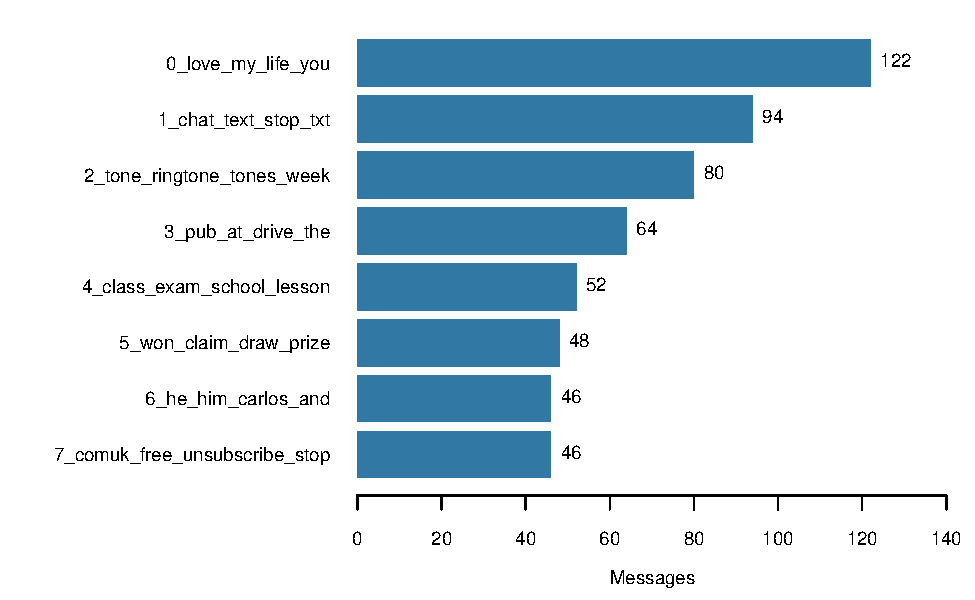
\includegraphics[width=0.98\linewidth]{figures/worked_example_topic_counts.pdf}
\caption{Eight largest non-outlier topics in the complete SMS worked example. Bars show message counts, and labels are the fitted model's automatic topic names. The figure uses the example's own archived topic metadata, before representation updates; these names are not substantive coding judgments. The controlled benchmark uses a separately configured vectorizer.}
\label{fig:worked_counts}
\end{figure}

\begin{lstlisting}[caption={Creating HTML visualizations and saving the fitted model.}]
bertopic_visualize_topics(
  model,
  file = "viz_topics.html"
)

bertopic_visualize_heatmap(
  model,
  file = "viz_heatmap.html"
)

# Topic representations can be recomputed after inspection.
bertopic_update_topics(model, docs)
updated_topic_info <- bertopic_topics(model)

# Save the fitted Python model; load only trusted serialized models.
bertopic_save(
  model,
  path = "sms_bertopic_model",
  serialization = "safetensors",
  overwrite = TRUE
)
restored_model <- bertopic_load("sms_bertopic_model")
restored_topic_info <- bertopic_topics(restored_model)
stopifnot(identical(
  as.data.frame(restored_topic_info)[c("Topic", "Count", "Name")],
  as.data.frame(updated_topic_info)[c("Topic", "Count", "Name")]
))
\end{lstlisting}

The complete worked example was rerun using the installed 0.1.2 source archive and pinned embedding-model revision. Its console output, numerical tables, HTML, Plotly JSON, and static figures were retained separately from the controlled benchmark. All six restoration checks passed: topic metadata after safetensors loading, and metadata, cached assignments, cached strengths, transformed assignments, and transformed strengths after a full pickle round trip. Lightweight formats omit the fitted reducer and clusterer, so metadata restoration does not establish identical HDBSCAN inference after lightweight loading. Full pickle reuse requires a matching environment and a trusted serialized model.

The SMS data contain no genuine time variable. We therefore do not interpret a topics-over-time analysis for this corpus. The functions \code{bertopic\_topics\_over\_time()} and \code{bertopic\_visualize\_topics\_over\_time()} are available for datasets with substantively meaningful timestamps.

\section{Comparison with the Python Implementation}
\label{sec:evaluation}

\subsection{Benchmark design}

Because the R and Python calls use the same Python library, a comparison of topic quality would not compare two different algorithms. We instead tested whether the R wrapper returned the same selected outputs as equivalent Python code and measured the additional runtime and memory used by the R process. This test does not assess whether BERTopic discovers substantively valid topics.

The benchmark used 2,247 SMS messages and installed \pkg{BERTopic} 0.1.2, tag \fcode{v0.1.2}, source commit \fcode{faee106}. The exact source archive checksum is retained with the outputs. Embeddings were generated once with \fcode{all-MiniLM-L6-v2} at immutable revision \fcode{1110a243fdf4706b3f48f1d95db1a4f5529b4d41}, then reduced from 384 to five dimensions with UMAP and \fcode{random_state = 42}. The frozen array was stored as float64 in column-major order to match R's conversion through \pkg{reticulate}. Both paths used \fcode{BaseDimensionalityReduction()}, HDBSCAN with \fcode{min_cluster_size = 10} and \fcode{prediction_data = TRUE}, an English-stop-word \fcode{CountVectorizer}, and \fcode{calculate_probabilities = TRUE}. Document and array SHA-256 hashes were \fcode{2f90a92a...fb036675} and \fcode{f8169618...92bc3531}; full hashes and preparation settings are retained in the manifest.

Five fresh Python processes and five fresh R processes ran on Windows x64 (build 26200), with 8 physical cores, 16 logical processors, and 15.9 GiB of physical memory visible to the operating system. The stack was R 4.4.1, Python 3.10.21, BERTopic 0.16.0, NumPy 1.26.4, scikit-learn 1.4.2, PyTorch 2.1.2+cpu, transformers 4.47.0, UMAP 0.5.5, and HDBSCAN 0.8.37. Process order alternated, with R first on odd repetitions. Both paths inherited \fcode{PYTHONHASHSEED = 42} and identical single-thread settings for OpenMP and common numerical libraries. Components were constructed before timing. Python used \code{time.perf\_counter()}; R used elapsed \code{proc.time()}. R fit timing includes wrapper validation and conversion. Cold-process time includes startup, imports, input loading, component construction, fitting, and output writing. Windows peak resident memory was read from \fcode{psutil.Process().memory_info().peak_wset}. These are workflow measurements, not a language-neutral microbenchmark.

\subsection{Comparison of model outputs}

The controlled model produced 50 non-outlier topics and 808 outlier messages (36.0\%). Table~\ref{tab:topic_examples} shows the eight largest topics. Terms are model outputs rather than author-assigned labels and do not validate behavioral constructs.

\begin{table}[htbp]
\centering
\caption{Largest Non-Outlier Topics in the Controlled SMS Model}
\label{tab:topic_examples}
\small
\begin{tabularx}{\linewidth}{>{\centering\arraybackslash}p{1.2cm}
                             >{\centering\arraybackslash}p{1.8cm}
                             >{\raggedright\arraybackslash}X}
\toprule
Topic & Messages & Four highest-weight terms \\
\midrule
0 & 122 & love, life, miss, smile \\
1 & 94 & chat, text, stop, sex \\
2 & 80 & tone, ringtone, tones, 8007 \\
3 & 64 & pub, drive, car, im \\
4 & 52 & class, exam, school, teaches \\
5 & 48 & won, draw, claim, prize \\
6 & 46 & carlos, hes, says, tyler \\
7 & 46 & unsubscribe, free, sms, goto \\
\bottomrule
\end{tabularx}
\begin{flushleft}
\footnotesize Note. Terms and counts are reproduced from the frozen-input benchmark output. Topic identifiers are arbitrary model labels.
\end{flushleft}
\end{table}

Table~\ref{tab:equivalence} reports the paired comparison. All five pairs returned matching 2,247 assignments, 808 outliers, \code{Topic}/\code{Count}/\code{Name} metadata in 51 rows (including the outlier topic), and 510 ordered top-ten term keys. Maximum absolute weight and membership-strength differences were \fcode{5e-16} and \fcode{4.86e-16}, below the $10^{-12}$ tolerance. Membership-strength matrices had dimensions $ 2247\times 50$.

\begin{table}[htbp]
\centering
\caption{Comparison of R and Python Outputs Across Five Paired Runs}
\label{tab:equivalence}
\begin{tabularx}{\linewidth}{>{\raggedright\arraybackslash}X
                             >{\centering\arraybackslash}p{2.5cm}
                             >{\centering\arraybackslash}p{2.5cm}
                             >{\raggedright\arraybackslash}p{2.6cm}}
\toprule
Output & Direct Python & R interface & Comparison \\
\midrule
Document assignments & 2247 & 2247 & Exact in 5/5 pairs \\
Outlier assignments & 808 & 808 & Exact \\
Topic-information rows & 51 & 51 & Exact \\
Non-outlier topics & 50 & 50 & Exact \\
Ordered top-term keys & 510 & 510 & Exact \\
Maximum c-TF--IDF difference & --- & --- & \texttt{5e-16} \\
Membership-strength dimensions & $2247\times50$ & $2247\times50$ & Exact \\
Maximum probability difference & --- & --- & \texttt{4.86e-16} \\
\bottomrule
\end{tabularx}
\end{table}

Under this configuration, the R wrapper and direct Python code produced the same selected outputs. The comparison does not imply that separate stochastic fits will always be identical, nor does it validate the substantive interpretation of the recovered topics.

\subsection{Runtime and memory use}

Table~\ref{tab:benchmark} reports medians and interquartile ranges from five fresh processes per interface. Median fitting took 0.630 seconds in Python and 4.810 seconds in R. Paired R-minus-Python differences had medians of 4.183 seconds for fitting, 11.400 seconds for cold-process time, and 200.0 MiB for peak memory. Paired-difference medians are summarized separately from medians for each interface.

\begin{table}[htbp]
\centering
\caption{Runtime and Peak-Memory Benchmark}
\label{tab:benchmark}
\begin{threeparttable}
\begin{tabular}{lccc}
\toprule
Interface & Fit time, s & Cold-process time, s & Peak RSS, MiB \\
\midrule
Direct Python & 0.630 [0.630, 0.633] & 16.950 [16.870, 16.960] & 402.2 [402.1, 402.4] \\
R interface & 4.810 [4.810, 4.830] & 28.300 [28.280, 28.410] & 602.9 [601.3, 604.9] \\
\bottomrule
\end{tabular}
\begin{tablenotes}
\footnotesize
\item Note. Values are medians [interquartile ranges] from five fresh processes. Embedding generation and UMAP reduction were performed once before the timed paired calls. RSS = resident set size.
\end{tablenotes}
\end{threeparttable}
\end{table}

Direct Python used less time and memory in this Windows configuration. Paired median differences were 4.183 seconds for fitting, 11.400 seconds for cold-process time, and 200.0 MiB for peak memory. Embedding generation and reduction were excluded. These five replications of one corpus and configuration do not establish general performance advantages.

\subsection{Reproducibility under stochastic fitting}

Matching results in the controlled comparison and reproducibility across independent model fits are different questions. UMAP, approximate neighbor search, transformer execution, and hardware-specific numerical libraries may introduce variation. Topic identifiers can also change when clusters are reordered, even if their content is similar. For reproducible analyses, users should (a) set R and Python seeds; (b) pass \code{random\_state} explicitly to stochastic components that expose it; (c) record the R and Python package versions and the selected interpreter; (d) save the fitted model; and (e) evaluate topic stability across seeds or reasonable specifications when substantive conclusions depend on the discovered topics. Comparisons across stochastic fits should align topics by their documents or representations rather than assuming that equal numeric identifiers denote equal topics.

\subsection{Package checks and archive reconstruction}

The exact 0.1.2 source archive passed \code{R CMD check --no-manual} on the tested Windows configuration with zero errors and zero warnings. The testthat entrypoint executed 159 expectations with no failures, warnings, or skips. The sole package-check NOTE concerned 341 marked UTF-8 strings in the demonstration data. These checks cover the exercised wrapper operations and regression cases; they do not establish support for every Python constructor configuration.

A separate confirmation run cloned the archived Git bundle into a new working directory and installed the same source archive into an isolated R library. It reused the validated Python environment and existing R dependencies, rather than repeating a clean dependency installation. All five paired output comparisons and all six example restoration checks passed; eleven numerical CSV exports from the example matched the formal retained outputs byte for byte. Confirmation timings are archived separately and do not replace the measurements in Table~\ref{tab:benchmark}. Topic-metadata CSV exports encode list columns as JSON-valued cells; numeric matrix exports retain ordinary CSV columns. An additional checkout with \fcode{core.autocrlf=false} verified that the corrected archive preserves the recorded input bytes independently of that Git setting.

\section{Availability, Installation, and Operational Guidance}

\subsection{Software availability}

The evaluation used \pkg{BERTopic} 0.1.2, source tag \fcode{v0.1.2} and commit \fcode{faee106}. Development source and issue tracking are at \url{https://github.com/Feng-Ji-Lab/BERTopic}; the CRAN project page is \url{https://CRAN.R-project.org/package=BERTopic}. Reproduction requires the \href{https://github.com/Feng-Ji-Lab/BERTopic/raw/64907e737025fe456d3673afcf0f467df4deb20d/provenance/releases/BERTopic_0.1.2.tar.gz}{exact retained source archive}, rather than an unspecified current repository release. Versioned analysis materials are public under \href{https://github.com/Feng-Ji-Lab/BERTopic/tree/analysis-v0.1.2-r1}{\fcode{analysis-v0.1.2-r1}}, including the corrected input archive and reconstruction scripts. A version-specific OSF/Zenodo DOI remains pending. The R interface is MIT-licensed; dependencies and other archived materials retain their respective rights.

\subsection{One-time backend setup}

All relative paths below refer to a checkout of the package's analysis materials. For the recorded Python configuration, create a new Windows Conda environment from the archived resolved specification before starting R:

\begin{lstlisting}[language={},caption={Creating the recorded Python environment from PowerShell.}]
conda env create --name r-bertopic-paper-012 --file provenance/windows-bertopic-0.16.0.yml
\end{lstlisting}

Install the retained R source archive and bind the named environment before Python is initialized:

\begin{lstlisting}[caption={Installing the tested R package and binding its Python backend.}]
install.packages("provenance/releases/BERTopic_0.1.2.tar.gz",
                 repos = NULL, type = "source")
library(BERTopic)

stopifnot(packageVersion("BERTopic") == "0.1.2")
use_bertopic_condaenv("r-bertopic-paper-012")
stopifnot(bertopic_available())
bertopic_session_info()
\end{lstlisting}

If another interpreter has already been initialized by \pkg{reticulate}, restart R before binding this environment. For general installation, \code{install\_py\_deps\_conda()} and the virtualenv helper consume the same declared requirements. Those declarations are distinct from the fully resolved Windows environment retained for this analysis; installing them later can select different transitive dependencies.

The benchmark and example session files record R 4.4.1, \pkg{reticulate} 1.45.0, and the R dependency versions used. The supplied R dependency installer bootstraps from current CRAN and is not a complete historical R lockfile. An identical R stack therefore requires restoring the recorded versions separately. Backend installation and first-use model downloads can require network access. The pinned embedding-model revision, frozen reduced array, interpreter settings, seeds, full Python distributions, and file hashes are recorded with the outputs.

\subsection{Common installation and runtime problems}

\begin{table}[htbp]
\centering
\caption{Common Installation and Runtime Problems}
\label{tab:diagnostics}
\begin{tabularx}{\linewidth}{>{\raggedright\arraybackslash}p{3.4cm}
                             >{\raggedright\arraybackslash}X
                             >{\raggedright\arraybackslash}p{3.7cm}}
\toprule
Observed problem & Likely cause & Recommended action \\
\midrule
\fcode{bertopic_available()} is false & BERTopic is absent from the active interpreter & Run \fcode{bertopic_session_info()}, verify the Python path, then run \fcode{install_py_deps()} \\
Requested environment differs from active Python & \pkg{reticulate} initialized too early & Restart R, call \code{use\_bertopic()} before importing another Python module \\
Transformer model cannot be downloaded & Network, cache, or model-hub access & Pre-download the model in the bound environment or supply precomputed embeddings \\
Model fits but results differ across runs & A stochastic component lacks an explicit state & Pass \code{random\_state} to UMAP or other relevant components and record all versions \\
Saved model cannot be restored elsewhere & Backend or serialization mismatch & Match versions and test the required post-load operation; lightweight files omit clustering components \\
\bottomrule
\end{tabularx}
\end{table}

\section{Discussion}

The controlled comparison establishes a limited but useful result: for the frozen inputs and core fitting and extraction path tested here, the R wrapper preserved the selected outputs of direct Python execution. The additional time and memory reflect the cost of running R together with an embedded Python interpreter, but the short controlled task is not representative of an end-to-end analysis that includes transformer inference and UMAP. The evidence therefore supports an input--output mapping claim, not a general claim about computational efficiency, topic quality, or the reliability of every exported helper.

The practical value of the interface lies in keeping the fitted Python model and its commonly used outputs inside an R project. Researchers can move topic assignments, terms, membership strengths, and visualizations into later R analyses without repeatedly exchanging intermediate files. This benefit is most relevant when data preparation, statistical modeling, graphics, and reporting are already conducted in R. Direct Python remains the simpler option for Python-centered projects, for immediate access to newly released upstream features, or when avoiding the memory cost of two runtimes is important. Researchers who prefer an R interface should also compare the object model, backend support, documentation, and tests of \pkg{BERTopic} with those of \pkg{bertopicr}; the present study does not establish the superiority of either package.

Cross-language convenience does not remove the need for software-version control. Python package resolution, compiled libraries, model downloads, and hardware differences can prevent the same code from running elsewhere. The use of \code{...} exposes advanced constructor arguments but cannot protect users from changed upstream signatures or incompatible component versions. The tested backend is pinned to Python BERTopic 0.16.0. A citable analysis should therefore record the exact R and Python environments, save component settings, verify model restoration, and archive the package source used for the results. Organizing research products as versioned R packages and preserving the associated materials can make those dependencies more visible \citep{vuorre2021sharing}.

The controlled benchmark covers one Windows configuration, one short-text corpus, BERTopic 0.16.0, and five timing replications; embedding generation and reduction are excluded. Package checks and archive reconstruction provide additional evidence about the exercised R wrappers, but do not extend the benchmark to other operating systems, backend releases, or all advanced configurations. The SMS illustration also does not establish substantive topic quality.

The substantive limits of unsupervised topic modeling are unchanged by the interface. A coherent list of top words does not establish that a topic is a reliable psychological construct. Short documents near cluster boundaries may move between a substantive topic and the outlier class under modest specification changes, and HDBSCAN-derived membership strengths are not automatically calibrated probabilities of theoretically defined categories. Behavioral applications should justify the unit of analysis and embedding model, report preprocessing and component choices, inspect multiple representative documents, assess stability across reasonable specifications, and validate any topic-derived measure against its intended use. Evaluations of behavioral text-mining methods similarly emphasize that convenient model output cannot substitute for task-specific validation against human judgments or other relevant criteria \citep{macanovic2024systematic}.

In its current form, \pkg{BERTopic} provides an R-oriented access layer whose selected fitting and extraction outputs agree with direct Python execution under the tested configuration. The retained model, R data structures, explicit environment selection, and checked persistence workflows support integration into an R project. The evidence supports these interface and workflow claims while leaving the validity of topic-derived behavioral measures to application-specific evaluation.

\section*{Declarations}

\textbf{Funding.} \todo{Insert complete funding statement or ``No funding was received for conducting this study.''}

\textbf{Competing interests.} \todo{Insert author-approved competing-interests statement.}

\textbf{Ethics approval.} Not applicable. The software demonstration analyzes an existing public dataset distributed with the package.

\textbf{Consent to participate.} Not applicable.

\textbf{Consent for publication.} Not applicable.

\textbf{Availability of data and materials.} The exact packaged SMS input, frozen reduced embeddings, preparation and analysis scripts, raw outputs, environment specification, restoration checks, figures, and manuscript materials are retained in the \href{https://github.com/Feng-Ji-Lab/BERTopic/tree/analysis-v0.1.2-r1}{versioned public analysis source}. Historical ham-selection reconstruction remains unresolved as noted in the example. \todo{Insert the published version-specific OSF/Zenodo archive DOI.}

\textbf{Code availability.} Development source is at \url{https://github.com/Feng-Ji-Lab/BERTopic}. The analyses used version 0.1.2, source tag \fcode{v0.1.2}, commit \fcode{faee106}, and the retained source archive identified by SHA-256 in the release record. Analysis scripts and provenance are versioned separately under \fcode{analysis-v0.1.2-r1}. \todo{Insert the published version-specific archive DOI for the exact source and analysis scripts.}

\textbf{Author contributions.} \todo{Complete an author-approved CRediT contribution statement. Ensure that manuscript authorship and package-development contributions are documented consistently.}

\section*{Open Practices Statement}

The package source, inputs used in the reported analyses, scripts, raw benchmark and example outputs, tables and figures, environment records, and reconstruction documentation are available as versioned GitHub analysis materials. The confirmation run reused an existing validated dependency environment, and the historical SMS selection mechanism is not yet reconstructable from the original source. A durable OSF/Zenodo DOI remains to be supplied. The software evaluation was not preregistered.

\printbibliography

\end{document}
